\chapter{Interpretace logistického regresního modelu}

\section{Úvod}

Předpokladem interpretace libovolného nakalibrovaného modelu je, že jsme schopni smysluplně interpretovat jeho odhadnuté parametry. Tato interpretace zahrnuje dva kroky - (a) odhad funkcionálního vztahu mezi závislou a nezávislou veličinou a (b) definování vhodné jednotky změny nezávislé veličiny.

První krok předpokládá, že vztah mezi závislou a nezávislou veličinou lze popsat pomocí lineární funkce. V případě jednorozměrného lineárního regresního modelu má tento vztah podobu $y(x) = \beta_0 + \beta_1 x$. V případě logistického regresního modelu je tento vztah definován na úrovni logit funkce, tj. jako $g(x) = \ln \left(\frac{\pi(x)}{1 - \pi(x)}\right) = \beta_0 + \beta_1 x$.

Co se druhého kroku týče, je v případě jednorozměrného lineárního regresního modelu koeficient $\beta_1$ definován jako změna hodnoty závislé veličiny pro jednotkovou změnu závislé veličiny, tj. $\beta_1 = y(x + 1) - y(x)$. Naproti tomu v případě logistického regresního modelu představuje koeficient $\beta_1$ změnu v logit funkci, tj. $\beta_1 = g(x + 1) - g(x)$.

\section{Nezávislá binární veličina}

Nezávislou veličinu nazýváme binární, pokud nabývá pouze dvou hodnot. V následujícím textu budeme předpokládat, že taková veličina nabývá hodnot 0 a 1. Změna v logit funkci tak má podobu
\begin{equation}
g(1) - g(0) = [\beta_0 + \beta_1] - [\beta_0] = \beta_1.
\end{equation}
Možné kombinace logistické pravděpodobnosti jsou ilustrovány tabulkou na obrázku (3.1).
\begin{figure}[htp]
\centering
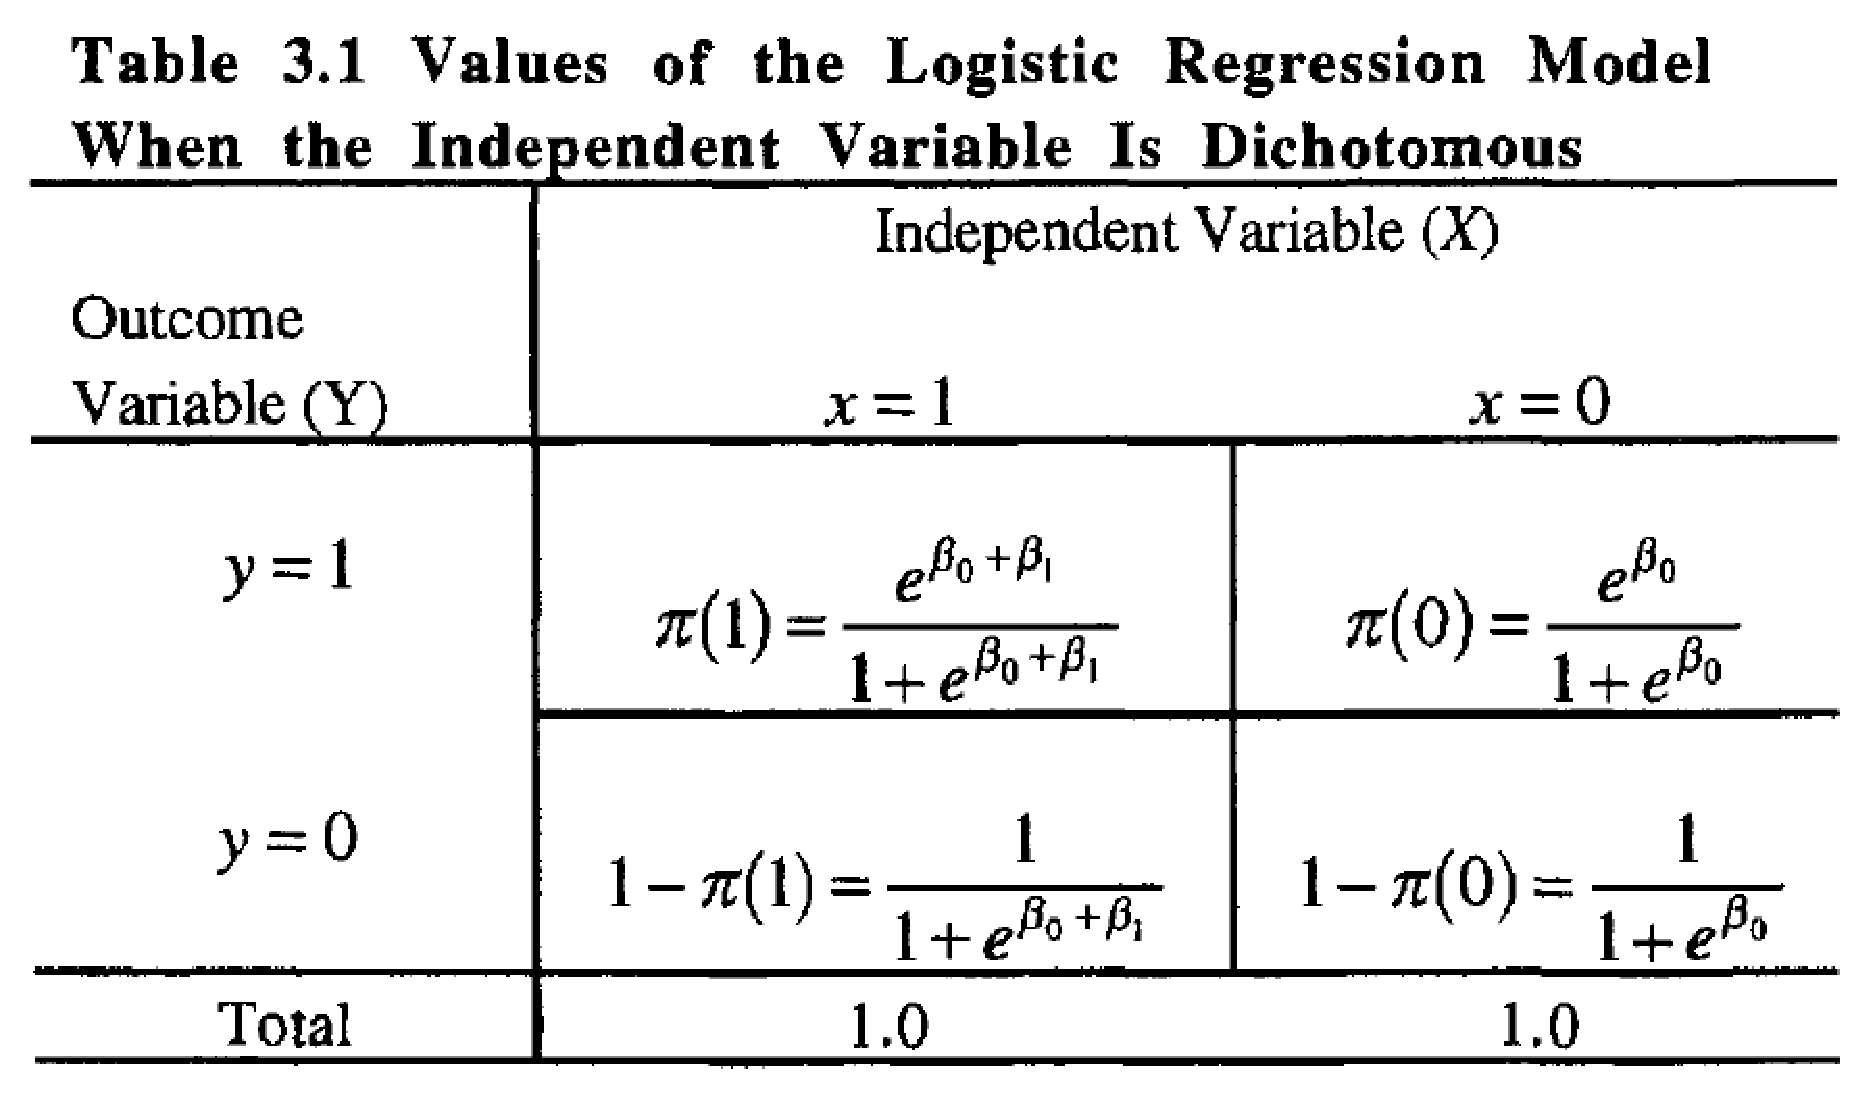
\includegraphics[scale = 0.35]{pictures/tbl_3_1.eps}
\caption{Hodnoty jednorozměrného logistického regresního modelu pro binární nezávislou veličinu}
\label{tbl_3_1}
\end{figure}

Důležitou statistikou používanou při analýze logistického regresního modelu je tzv. podíl rizik (odd ratio), které je definovaný jako
\begin{equation}
OR = \frac{\pi(1) / [1 - \pi(1)]}{\pi(0) / [1 - \pi(0)]}.
\end{equation}
V případě jednorozměrné logistické regrese s binární nezávislou veličinou, která nabývá hodnot 0 nebo 1, je vztah mezi podílem rizik a hodnotou regresního parametru definován jako
\begin{equation}
OR = \frac{\pi(1) / [1 - \pi(1)]}{\pi(0) / [1 - \pi(0)]} = \frac{\frac{e^{\beta_0 + \beta_1}}{1 + e^{\beta_0 + \beta_1}} \Big/ \frac{1}{1 + e^{\beta_0 + \beta_1}}}{\frac{e^{\beta_0}}{1 + e^{\beta_0}} \Big/ \frac{1}{1 + e^{\beta_0}}} = \frac{e^{\beta_0 + \beta_1}}{e^{\beta_0}} = e^{(\beta_0 + \beta_1) - \beta_0} = e^{\beta_1}.
\end{equation}
Podíl rizik přibližně vyjadřuje kolikrát je pravděpodobnější výskyt pozitivní hodnoty závislé veličiny pro pozorování $x = 1$ než pro pozorování $x = 0$. Pokud např. $y$ označuje výskyt / absenci rakoviny plic $x$ obsahuje informaci o tom, zda-li je daná osoba kuřák, pak $\widehat{OR} = 2$ znamená, že pravděpodobnost výskytu rakoviny plic u kuřáka je dvakrát vyšší než u nekuřáka. Vzhledem k definici podílu rizik je zřejmé, že tato statistika přibližně vyjadřuje tzv. relativní riziko, které je definováno jako $\pi(1) / \pi(0)$. Z tabulky (3.1) je pak zřejmé, že tato aproximace platí, pokud $[1 - \pi(0)] / [1 - \pi(1)] \approx 1$. To je splněno, pokud $\pi(x)$ je malé jak pro $x = 1$ tak pro $x = 0$.

V řadě aplikací logistické regrese, se kterými se můžeme setkat v odborné literatuře, jsou spojité numerické veličiny převedeny na binární pomocí vhodně zvoleného hraničního bodu. Pro ilustraci uvádíme klasifikační tabulku (3.2), kdy veličina $AGED$ nabývá hodnoty 0 pokud je dané osobě méně než 55 let a hodnoty 1 v ostatních případech.
\begin{figure}[htp]
\centering
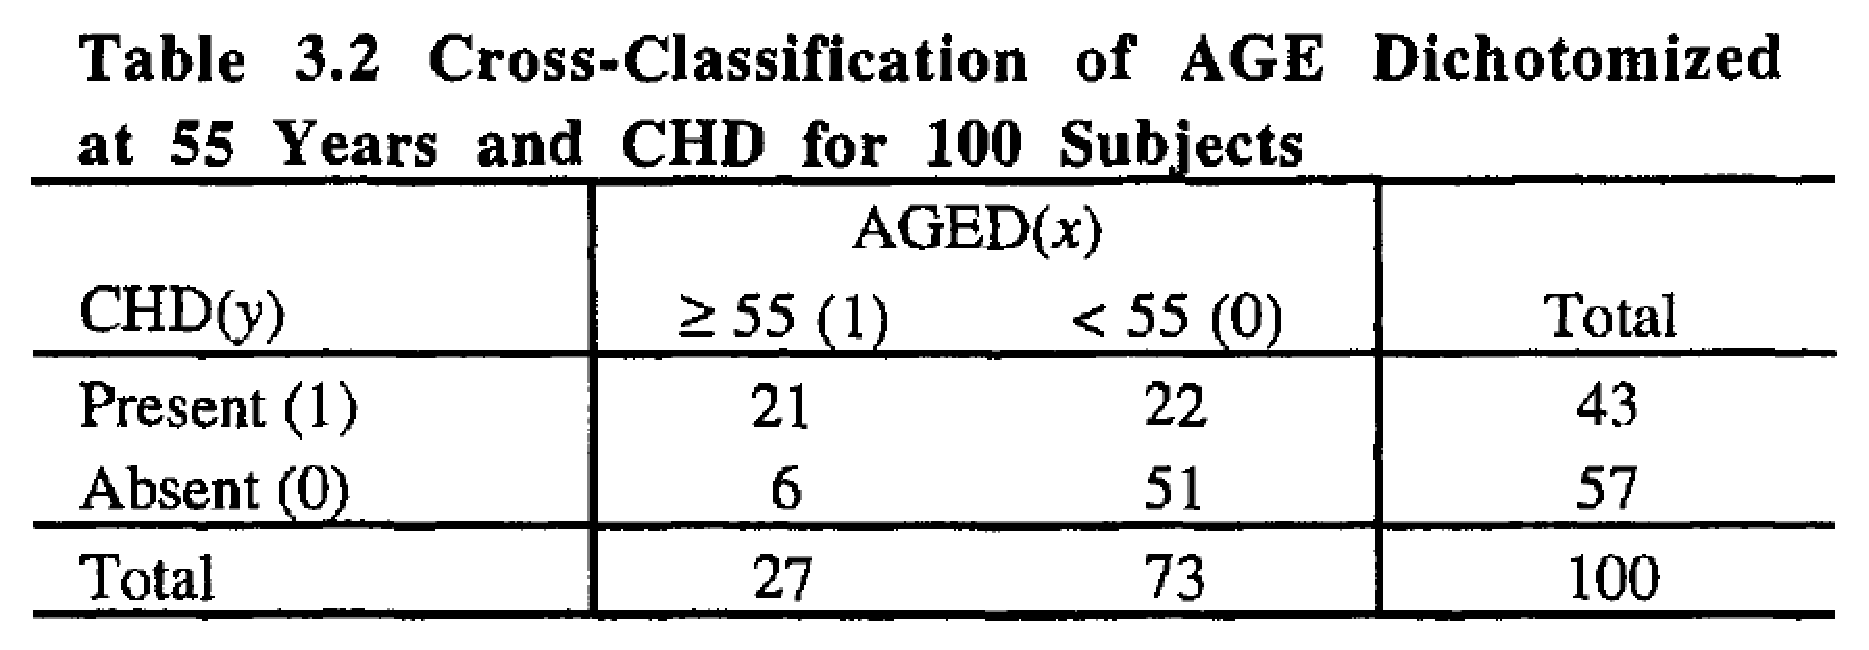
\includegraphics[scale = 0.35]{pictures/tbl_3_2.eps}
\caption{Klasifikační tabulka pro binární nezávislou veličinu $AGED$ a závislou veličinu $CHD$ představující výskyt ischemické choroby srdeční.}
\label{tbl_3_2}
\end{figure}
Zkoumaná populace se dle tabulky (3.2) skládala z 21 osob s hodnotami $(x = 1, y = 1)$, 22 osob s hodnotami $(x = 0, y = 1)$, 6 osob s hodnotami $(x = 1, y = 0)$ a 51 osob s hodnotami $x = 0, y = 0$. Pokud bychom na základě těchto dat odhadli metodou maximální věrohodnosti parametr pro veličinu $AGED$, získali bychom hodnotu 2.094. Podíl rizik bychom pak odhadli na $\widehat{OR} = e^{2.094} = 8.1$. Podíl rizik však lze odhadnout také přímo s pomocí klasifikační tabulky, tj. jako
\begin{equation}
\widehat{OR} = \frac{\hat{\pi}(1) / [1 - \hat{\pi}(1)]}{\hat{\pi}(0) / [1 - \hat{\pi}(0)]} = \frac{21/6}{22/51} = 8.11.
\end{equation}
Interval spolehlivosti podílu rizik se pak určí tak, že se nejprve vypočtou krajní hodnoty odpovídající intervalu spolehlivosti odhadu parametru $\beta_1$ a na ně se aplikuje exponenciála, tj.
\begin{equation}
e^{\beta_1 \pm z_{1 - \alpha / 2} \widehat{se}(\hat{\beta}_1)}.
\end{equation}
Vzhledem ke způsobu konstrukce je interval spolehlivosti podílu rizik nesymetrický.

V předchozím textu jsme předpokládali, že nezávislá binární veličina $x$ nabývá veličin 0 a 1. Je třeba zdůraznit, že výše uvedené závěry jsou platné pouze pro tento případě. Uvažujme situaci, kdy $x$ nabývá dvou různých obecných hodnot $a$ a $b$. Pak platí
\begin{equation}
\ln[\widehat{OR}(a, b)] = \hat{g}(x = a) - \hat{g}(x = b) = (\hat{\beta}_0 + \hat{\beta}_1 a) - (\hat{\beta}_0 + \hat{\beta}_1 b) = \hat{\beta}_1 (a - b)
\end{equation}
neboli
\begin{equation}
\widehat{a, b} = e^{\hat{\beta}_1 (a - b)}.
\end{equation}
Analogie (3.2) pak má podobu
\begin{equation}
\widehat{OR}(a, b) = \frac{\hat{\pi}(x = a) / [1 - \hat{\pi}(x = a)]}{\hat{\pi}(x = b) / [1 - \hat{\pi}(x = b)]}.
\end{equation}
Interval spolehlivosti podílu rizik lze vyjádřit jako
\begin{equation}
e^{\hat{\beta}_1(a - b) \pm z_{1 - \alpha / 2}|a - b| \widehat{se}(\hat{\beta}_1)}.
\end{equation}
Je třeba zdůraznit, že kódování binární proměnné do 0 a 1 je zdaleka nejčastější, a proto ho budeme používat i v následujícím textu. Dalším používaným kódováním je pak -1 a 1, které je však méně frekventované.

\section{Nezávislá kategorická veličina}

Kategorickou veličinou rozumíme veličinu, která může nabývat $k > 2$ různých nominální hodnot. Jak jsme již zmínili výše, takovouto veličinu musíme převést na $k - 1$ pomocných binárních veličin. Jako příklad uveďme veličinu $X_i$, která nabývá hodnot 0 pro bělocha, 1 pro černocha a 2 pro asiata. Tuto veličinu musíme nahradit dvojicí pomocných binárních veličin $D_{i1}$ a $D_{i2}$. Při nejčastěji používaném kódování nabývá veličina $D_{i1}$ hodnoty 1, pokud je daná osoba černoch, a 0 v ostatních případech. Podobně veličina $D_{i2}$ nabývá hodnoty 1, pokud je daná osoba asiat, a 0 v ostatních případech. Je třeba zdůraznit, že pokud bych do modelu přidali ještě třetí veličinu, $D_{i3}$, která by nabývala hodnoty 1, pokud je daná osoba běloch, a 0 v ostatních případech, vytvořili bychom perfektní multikolinearitu.\footnote{Informaci o tom, že je daná osoba běloch totiž, lze získat také na základě veličin $D_{i1}$ a $D_{i2}$. Konkrétně, pokud obě veličiny nabývají hodnoty 0, víme, že se nejedná ani o černocha a ani o asiata, takže se musí jednat o bělocha. Informace představovaná veličinou $D_{i3}$ je tak duplicitní.}

Pro ilustraci uvažujme model $y(\pmb{x}) = \beta_0 + \beta_1 D_{i1} + \beta_2 D_{i2}$, kde $y = 1$ představuje výskyt ischemické choroby srdeční. Pokud použijeme standardní kódování pomocných binárních veličin na hodnoty 0 a 1, platí
\begin{equation}
\ln[\widehat{OR}(\textit{black}, \textit{white})] = \hat{g}(\textit{black}) - \hat{g}(\textit{white}) = (\hat{\beta}_0 + \hat{\beta}_1 \cdot 1 + \hat{\beta}_2 \cdot 0) - (\hat{\beta}_0 + \hat{\beta}_1 \cdot 0 + \hat{\beta}_2 \cdot 0) = \hat{\beta}_1.
\end{equation}
Jak vyplývá z označení $\widehat{OR}(\textit{black}, \textit{white})$, vyjadřuje $\hat{\beta}_1$ odhad, kolikrát je výskyt ischemické choroby srdeční pravděpodobnější u černocha než u bělocha.  Pokud bychom chtěli porovnat pravděpodobnosti výskytu ischemické choroby srdeční pro černocha vs. asiata, museli bychom výše uvedenou rovnici upravit do tvaru
\begin{multline}
\ln[\widehat{OR}(\textit{black}, \textit{asian})] = \hat{g}(\textit{black}) - \hat{g}(\textit{asian}) =\\(\hat{\beta}_0 + \hat{\beta}_1 \cdot 1 + \hat{\beta}_2 \cdot 0) - (\hat{\beta}_0 + \hat{\beta}_1 \cdot 0 + \hat{\beta}_2 \cdot 1) = \hat{\beta}_1 - \hat{\beta}_2.
\end{multline}
Interval spolehlivosti $\widehat{OR}(\textit{black}, \textit{white})$ pak má podobu
\begin{equation}
e^{\hat{\beta}_1 \pm z_{1 - \alpha / 2} \sqrt{\widehat{var}\big(\ln[\widehat{OR}(\textit{black}, \textit{white})]\big)}} = e^{\hat{\beta}_1 \pm z_{1 - \alpha / 2} \widehat{se}(\hat{\beta}_1)}
\end{equation}
a interval spolehlivosti $\widehat{OR}(\textit{black}, \textit{asian})$ podobu
\begin{equation}
e^{(\hat{\beta}_1 - \hat{\beta}_2) \pm z_{1 - \alpha / 2} \sqrt{\widehat{var}\big(\ln[\widehat{OR}(\textit{black}, \textit{asian})]\big)}},
\end{equation}
kde
\begin{equation}
\widehat{var}\big(\ln[\widehat{OR}(\textit{black}, \textit{asian})]\big) = \widehat{var}(\hat{\beta}_1) - 2 \hat{\beta}_1 \hat{\beta}_2 \widehat{cov}(\hat{\beta}_1, \hat{\beta}_2) + \widehat{var}(\hat{\beta}_2).
\end{equation}

Dalším možným způsobem kódování je použití hodnot -1, 0 a 1. Běloch je tak reprezentován hodnotami -1 pro $D_{i1}$ a -1 pro $D_i2$, černoch hodnotami 1 pro $D_{i1}$ a 0 pro $D_{i2}$ a konečně asiat hodnotami 0 pro $D_{i1}$ a 1 pro $D_{i2}$. Platí tedy
\begin{equation}
\ln[\widehat{OR}(\textit{black}, \textit{white})] = \hat{g}(\textit{black}) - \hat{g}(\textit{white}) = (\hat{\beta}_0 + \hat{\beta}_1 \cdot 1 + \hat{\beta}_2 \cdot 0) - (\hat{\beta}_0 + \hat{\beta}_1 \cdot (-1) + \hat{\beta}_2 \cdot (-1)) = 2\hat{\beta}_1 + \hat{\beta}_2
\end{equation}
a podobně
\begin{equation}
\ln[\widehat{OR}(\textit{black}, \textit{asian})] = \hat{g}(\textit{black}) - \hat{g}(\textit{asian}) = (\hat{\beta}_0 + \hat{\beta}_1 \cdot 1 + \hat{\beta}_2 \cdot 0) - (\hat{\beta}_0 + \hat{\beta}_1 \cdot 0 + \hat{\beta}_2 \cdot 1) = \hat{\beta}_1 - \hat{\beta}_2
\end{equation}.
Intervaly spolehlivosti podílů rizik pak mají podobu
\begin{equation}
e^{(2\hat{\beta}_1 + \hat{\beta}_2) \pm z_{1 - \alpha / 2} \sqrt{\widehat{var}\big(\ln[\widehat{OR}(\textit{black}, \textit{white})]\big)}}
\end{equation}
pro $\widehat{OR}(\textit{black}, \textit{white})$ a
\begin{equation}
e^{(\hat{\beta}_1 - \hat{\beta}_2) \pm z_{1 - \alpha / 2} \sqrt{\widehat{var}\big(\ln[\widehat{OR}(\textit{black}, \textit{asian})]\big)}}
\end{equation}
pro $\widehat{OR}(\textit{black}, \textit{asian})$ kde
\begin{equation}
\widehat{var}\big(\ln[\widehat{OR}(\textit{black}, \textit{white})]\big) = 4\widehat{var}(\hat{\beta}_1) + 4 \hat{\beta}_1 \hat{\beta}_2 \widehat{cov}(\hat{\beta}_1, \hat{\beta}_2) + \widehat{var}(\hat{\beta}_2).
\end{equation}
a
\begin{equation}
\widehat{var}\big(\ln[\widehat{OR}(\textit{black}, \textit{asian})]\big) = \widehat{var}(\hat{\beta}_1) - 2 \hat{\beta}_1 \hat{\beta}_2 \widehat{cov}(\hat{\beta}_1, \hat{\beta}_2) + \widehat{var}(\hat{\beta}_2).
\end{equation}
Tento způsob kódování je však používán spíše výjimečně, a proto budeme v následujícím textu používat kódování pomocí hodnot 0 a 1.